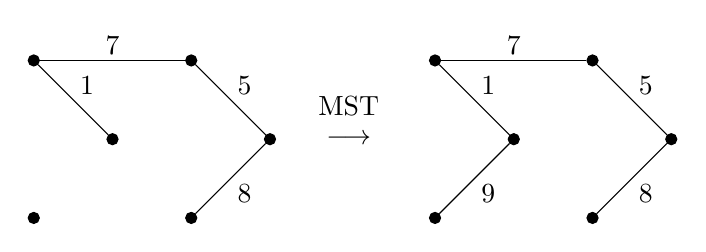
\begin{tikzpicture}[black/.style={circle,draw,fill=black,inner sep=0pt, minimum width=4pt}]
	\foreach \x in {0,2}
		\node[black,xshift=145] at (\x,2) (a\x) {};
	\foreach \x in {1,3}
		\node[black,xshift=145] at (\x,1) (b\x) {};
	\foreach \x in {0,2}
		\node[black,xshift=145] at (\x,0) (c\x) {};
	\draw (a0) -- (a2) node [midway,label={7},yshift=-5] {};
	% \draw (c0) -- (c2) node [midway,label=below:{15},yshift=5] {};
	% \draw (a0) -- (c0) node [midway,label=left:{13},xshift=5] {};
	% \draw (a2) -- (c2) node [midway,label=right:{18},xshift=-5] {};
	\draw (a0) -- (b1) node [midway,label={1},xshift=5,yshift=-5] {};
	% \draw (a2) -- (b1) node [midway,label={12},xshift=-5,yshift=-5] {};
	\draw (c0) -- (b1) node [midway,label=below:{9},xshift=5,yshift=5] {};
	% \draw (c2) -- (b1) node [midway,label=below:{11},xshift=-5,yshift=5] {};
	\draw (a2) -- (b3) node [midway,label={5},xshift=5,yshift=-5] {};
	\draw (c2) -- (b3) node [midway,label=below:{8},xshift=5,yshift=5] {};


	\draw node at (4,1) {$\longrightarrow$};
	\draw[above,yshift=5] node at (4,1) {MST};


	\foreach \x in {0,2}
		\node[black] at (\x,2) (a\x) {};
	\foreach \x in {1,3}
		\node[black] at (\x,1) (b\x) {};
	\foreach \x in {0,2}
		\node[black] at (\x,0) (c\x) {};
	\draw (a0) -- (a2) node [midway,label={7},yshift=-5] {};
	% \draw (c0) -- (c2) node [midway,label=below:{15},yshift=5] {};
	% \draw (a0) -- (c0) node [midway,label=left:{13},xshift=5] {};
	% \draw (a2) -- (c2) node [midway,label=right:{18},xshift=-5] {};
	\draw (a0) -- (b1) node [midway,label={1},xshift=5,yshift=-5] {};
	% \draw (a2) -- (b1) node [midway,label={12},xshift=-5,yshift=-5] {};
	% \draw (c0) -- (b1) node [midway,label=below:{9},xshift=5,yshift=5] {};
	% \draw (c2) -- (b1) node [midway,label=below:{11},xshift=-5,yshift=5] {};
	\draw (a2) -- (b3) node [midway,label={5},xshift=5,yshift=-5] {};
	\draw (c2) -- (b3) node [midway,label=below:{8},xshift=5,yshift=5] {};
\end{tikzpicture}
